\setAuthor{Valter Kiisk}
\setRound{piirkonnavoor}
\setYear{2005}
\setNumber{G 1}
\setDifficulty{2}
\setTopic{Kinemaatika}

\prob{Veok}
Veok sõidab maanteel ühtlase kiirusega $v_1 = \SI{80}{km/h}$. Veokile järgneb $l_1 = \SI{10}{m}$ kaugusel sõiduauto. Veoki pikkus on $L_1 = \SI{12}{m}$, sõiduauto pikkus $L_2 = \SI{4}{m}$. Sõiduauto sooritab möödasõidu ühtlase kiirendusega $a = \SI{2}{m/s^2}$. Möödasõit lõpeb siis, kui sõiduauto on veokist $l_2 = \SI{10}{m}$ kaugusel. Kui pikas minimaalses ulatuses $s$ peaks vastassuunaline rada vaba olema ohutuks möödasõiduks? Ohutuks kauguseks vastutulevast autost loetakse $l_3 = \SI{30}{m}$. Vastutulevad autod sõidavad kiirusega $v_2 = \SI{90}{km/h}$.

\begin{center}
	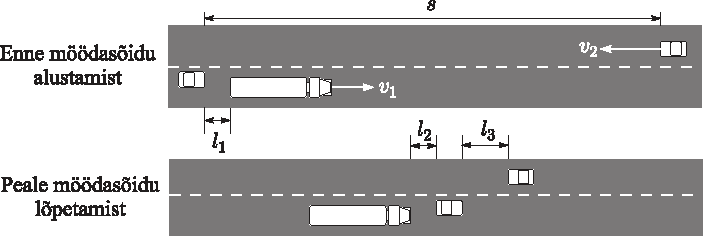
\includegraphics[width=\linewidth]{2005-v2g-01-yl}
\end{center}

\hint
Möödasõidu käigus avaldub sõiduauto läbitud vahemaa ühtlase kiirenduse valemiga $x = vt + \frac{at^2}{2}$.

\solu
Tähistagu $x$ teepikkust, mille sõiduauto läbib möödasõidu lõpuks (vt joonist) ja olgu $t$ möödasõiduks kuluv ajavahemik. Vahemaa $x$ läbib sõiduauto ühtlase kiirendusega $a$, alustades algkiirusega $v_1$, seega
\[
x = v_1t + \frac{at^2}{2}. 
\]
Teiselt poolt, veoauto liikumise põhjal
\[
x = v_1t + L_1 + L_2 + l_1 + l_2.
\]
Kahe viimase avaldise võrdsustamisel saame
\[
\frac{a t^{2}}{2}=L_{1}+L_{2}+l_{1}+l_{2} \Rightarrow t=\sqrt{\frac{2\left(L_{1}+L_{2}+l_{1}+l_{2}\right)}{a}}\Rightarrow
\]
\[
\begin{aligned}
s &= v_1t + L_1 + L_2 + l_1 + l_2 + v_2t + l_3\\
s &= \left(v_{1}+v_{2}\right) \sqrt{\frac{2\left(L_{1}+L_{2}+l_{1}+l_{2}\right)}{a}}+L_{1}+L_{2}+l_{1}+l_{2}+l_{3} \approx \SI{349}{m}
\end{aligned}
\]

\begin{center}
	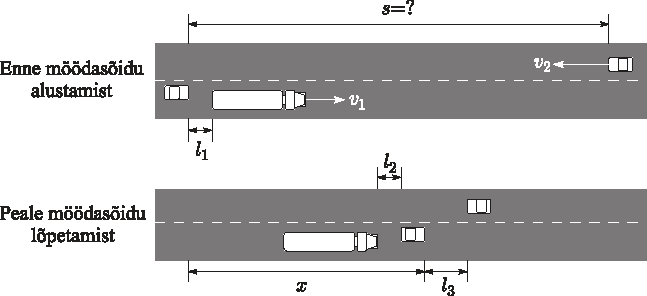
\includegraphics[width=\linewidth]{2005-v2g-01-lah}
\end{center}

\emph{Alternatiivne lahendus}

Kasutame möödasõidu aja leidmiseks veoauto taustsüsteemi, kus möödasõitva auto
algkiirus on $u = 0$:
\[
\frac{at^2}{2} = L_1 + L_2 + l_1 + l_2.
\]
Selle aja jooksul lähenevad veoauto ja vastutulev auto vahemaa
\[
s_1 = (v_1 + v_2)t 
\]
võrra, mis tähendab, et möödasõitja algvahemaa on
\[
s = s_1 + L_1 + L_2 + l_1 + l_2 + l_3 ,
\]
st (asendades $s_1$ ja $t$ eelnevatest võrranditest)
\[
s=\left(v_{1}+v_{2}\right) \sqrt{\frac{2\left(L_{1}+L_{2}+l_{1}+l_{2}\right)}{a}}+L_{1}+L_{2}+l_{1}+l_{2}+l_{3} \approx \SI{349}{m}.
\]
\probend